\documentclass[11pt,answers]{exam}
\usepackage[margin=1in, a4paper]{geometry}

\usepackage{amsmath, amssymb, amsthm, amsbsy, amsfonts, mathtools}
\usepackage{siunitx}

\usepackage{tikz, pgfplots}
\pgfplotsset{compat=1.16}
\usepackage{graphicx}

\usepackage{setspace}
\usepackage{cancel}
\usepackage{cases}
\usepackage[nolabel, final]{showlabels}

\usepackage{fourier}
\usepackage{plex-serif}
\usepackage[basic,italic,symbolgreek]{mathastext}
\makeatletter
\@for\@tempa:=a,b,c,d,e,h,i,k,l,m,n,o,q,r,s,t,u,v,w,x\do{%
\MTsetmathskips{\@tempa}{0.5mu}{0.5mu}}%
\makeatother
\MTsetmathskips{f}{2.5mu}{0.5mu}
\MTsetmathskips{g}{1.5mu}{0.5mu}
\MTsetmathskips{j}{2.5mu}{0.5mu}
\MTsetmathskips{p}{1.5mu}{0mu}
\MTsetmathskips{y}{1.5mu}{0.5mu}
\MTsetmathskips{z}{1mu}{0.5mu}

\newcommand{\reals}{\mathbb{R}}
\newcommand{\ints}{\mathbb{Z}}
\newcommand{\posints}{\mathbb{Z}^{+}}
\newcommand{\rationals}{\mathbb{Q}}
\newcommand{\complexes}{\mathbb{C}}
\renewcommand{\frac}[2]{\dfrac{#1}{#2}}
\newcommand{\oneover}[1]{\dfrac{1}{#1}}
\newcommand{\qndate}[2]{(\textbf{#1 #2})}

\pagestyle{plain}

\begin{document}
\doublespacing%

\begin{center}
	\Large
	\textbf{Problem Of The Day 2022}
\end{center}

\begin{questions}
	\question \qndate{27}{Jun} If $y$ varies inversely as $x$ and can be
	represented by the equation $y = (m-1){x}^{m^2 - 2}$, find the value of
	constant $m$.
	\begin{solution}
		\begin{align*}
			y = (m-1){x}^{m^2 - 2} & = \frac{k}{x}                                    \\
			k                      & = (m-1){x}^{m^2-1}                               \\
			                       & = (m-1){x}^{(m+1)(m-1)} \: \left(x \neq 0\right) \\
		\end{align*}
		By definition, $y \neq 0$ as well, hence
		\begin{align*}
			(m-1){x}^{(m+1)(m-1)} & \neq 0 \\
			\therefore m          & \neq 1
		\end{align*}
	\end{solution}


	\question \qndate{28}{Jun} Which of the following is a possible plot of
	$y = x + m$ and $y = \frac{m}{x}$ on the same axes? (The graphs are not drawn
	to scale.)
	\begin{figure}[htpb]
		\centering
		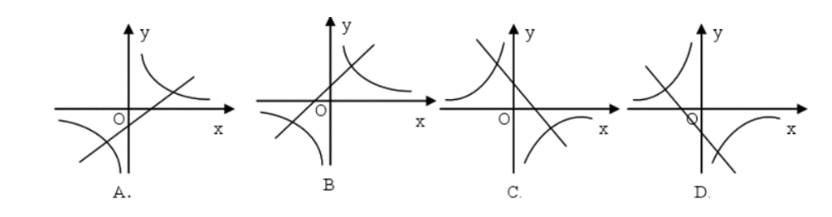
\includegraphics[scale=.8]{./images/0628_Graphs.png}
		\caption{$y = x + m$ and $y = \frac{m}{x}$.}
		\label{fig:0628_Graphs}
	\end{figure}
	\begin{solution}
		\textbf{B}.
		\begin{itemize}
			\item The straight line should be increasing, since the coefficient of $x$ is positive.
			      \textbf{C} and \textbf{D} are eliminated.
			\item If $m > 0$, the y-intercept of the straight line could not be negative.
			      \textbf{A} is eliminated, since the hyperbola in the same graph shows that $m>0$.
		\end{itemize}
	\end{solution}


	\question \qndate{29}{Jun} Given that points $A\left(-2,y_1\right)$, $B\left(-1,y_2\right)$,
	$C\left(1,y_3\right)$ are all on the graph of $y=-\oneover{x}$, arrange $y_1$,
	$y_2$ and $y_3$ in ascending order.
	\begin{solution}
		$y_3 < y_1 < y_2$.

		Subst. $x = -2$ into $y=-\oneover{x}$:
		\begin{align*}
			y_1 & = -\oneover{-2} \\
			    & = \oneover{2}
		\end{align*}

		Subst. $x=-1$ into $y=-\oneover{x}$:
		\begin{align*}
			y_2 & = -\oneover{-1} \\
			    & = 1
		\end{align*}

		Subst $x=1$ into $y=-\oneover{x}$:
		\begin{align*}
			y_3 & = -\oneover{1} \\
			    & = -1
		\end{align*}
	\end{solution}


	\question \qndate{30}{Jun} Given that points $\left(x_1,y_1\right)$, $\left(x_2,y_2\right)$
	and $\left(x_3,y_3\right)$ are all on the graph of $y=\frac{3}{x}$, also
	$x_1<x_2<0<x_3$, arrange $y_1$, $y_2$ and $y_3$ in ascending order.
	\begin{solution}
		$y_2<y_1<y_3$.
		\begin{itemize}
			\item $y_3 > 0$ since $x_3 > 0$. Hence, $y_3$ is the greatest.
			\item $0 > x_2 > x_1$, hence $y_2 < y_1 < 0$.
		\end{itemize}
	\end{solution}

	\question \qndate{1}{Jul} Given that $y$ varies inversely as $x$ such that
	$y = \left(a-2\right){x}^{a^2-5}$, also when $x>0$, as $x$ increases, $y$
	increases. Find the equation of the hyperbola.
	\begin{solution}
		\begin{align*}
			\frac{k}{x}                                 & = \left(a-2\right){x}^{a^2-5}                                                       \\
			k                                           & = \left(a-2\right){x}^{a^2-4}                                                       \\
			                                            & = \left(a-2\right){x}^{(a+2)(a-2)}                                                  \\
			\because y                                  & = \frac{\left(a-2\right){x}^{(a+2)(a-2)}}{x}                                        \\
			\therefore \left(a-2\right){x}^{(a+2)(a-2)} & < 0                                                                                 \\
			\because a - 2 < 0                          & \text{ and } (a+2)(a-2) \geq 0                                                      \\
			\therefore a + 2                            & = 0                                                                                 \\
			\therefore a                                & = -2                                                                                \\
			\therefore y                                & = -\frac{\left(-2-2\right)\times {x}^{\left(-2+2\right)\times\left(-2-2\right)}}{x} \\
			                                            & = -\frac{4}{x}
		\end{align*}
	\end{solution}

	\question \qndate{5}{Jul} If a straight line $y = (2m - 1)x$ and a hyperbola
	$y = \frac{3-m}{x}$ has an intersection point each in Quadrant 1 and 3, what
	is the range of values of the constant $m$?
	\begin{solution}
		\begin{align*}
			\because y        & = \frac{3-m}{x} \\
			\therefore m      & < 3             \\
			\because y        & = x(2m - 1)     \\
			\therefore 2m - 1 & > 0             \\
			\therefore 0.5    & < m < 3
		\end{align*}
	\end{solution}

	\question Points $A$ and $B$ are on the hyperbola $y = \frac{k}{x}$. Right $\triangle AOC$
	and $\triangle BOD$ are drawn by perpendicular lines drawn from the two points and connecting
	the points with the origin. Compare the sizes of the areas of the two triangles.
	\begin{figure}[htpb]
		\centering
		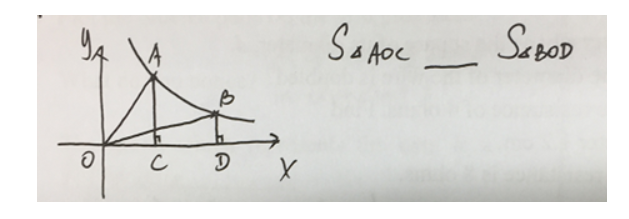
\includegraphics[scale=.8]{./images/0706_Tri.png}
		\caption{$\triangle AOC$ and $\triangle BOD$.}
		\label{fig:0706_Tri}
	\end{figure}
	\begin{solution}
		$S_{\triangle AOC} < S_{\triangle BOD}$.

		As Point $B$'s $y$-coordinate approaches 0, its $x$-coordinate approaches infinity,
		resulting in a triangle which approaches an infinite area. Point $A$ is further from
		$(\infty, 0)$ than Point $B$, so $S_{\triangle AOC} < S_{\triangle BOD}$.
	\end{solution}

	\question \qndate{7}{Jul} Points $A$ and $B$ are on the hyperbola $y = \frac{3}{x}$.
	Rectangles are drawn from the two points as shown. The areas bounded by the two
	rectangles are labelled $S_1$ and $S_2$. If the shaded area is 1 sq. unit, find
	the sum $S_1 + S_2$.
	\begin{figure}[htpb]
		\centering
		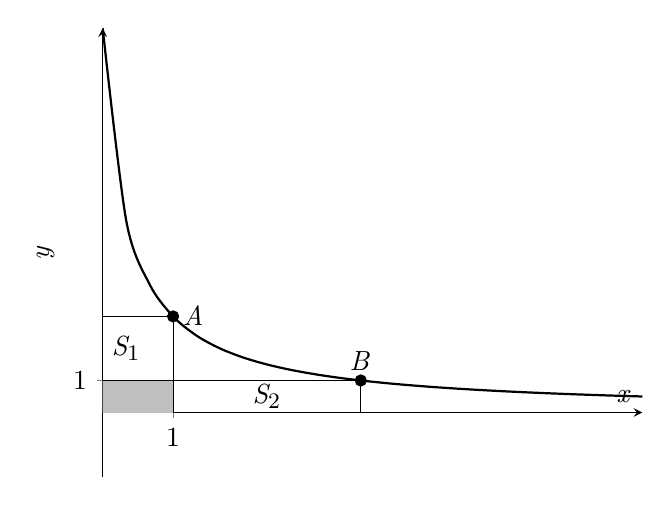
\begin{tikzpicture}
			\begin{axis}[
					domain=0:6,
					smooth,
					axis x line=center,
					axis y line=left,
					xlabel=$x$,
					ylabel=$y$,
					xtick={1},
					ytick={1},
					ymin=-2,
					scaled ticks=true,
				]
				\addplot[black,thick] {3/x};
				\filldraw (1,3) circle[radius=2pt] node[right]{$A$};
				\filldraw (3,1) circle[radius=2pt] node[above]{$B$};
				\filldraw[lightgray] (0,0) rectangle (1,1);
				\draw (0,1) rectangle (1,3) node[pos=.5]{$S_1$};
				\draw (1,0) rectangle (3,1) node[pos=.5]{$S_2$};
			\end{axis}
		\end{tikzpicture}
		\caption{The shaded areas, $S_1$ and $S_2$.}
		\label{fig:0707_Hyper}
	\end{figure}
	\begin{solution}
		\begin{align*}
			S_1       & = \left(1 - 0\right) \times \left(\frac{3}{1}-1\right)   \\
			          & = 2 \text{ sq. units}                                    \\
			S_2       & = \left(\frac{3}{3} - 0\right) \times \left(3 - 1\right) \\
			          & = 2 \text{ sq. units}                                    \\
			S_1 + S_2 & = 2 + 2                                                  \\
			          & = 4 \text{ sq. units}
		\end{align*}
	\end{solution}
\end{questions}
\end{document}
